\section{Library Structures}
\begin{frame}
  \begin{center}
    {\large Lecture 02 -- Data Structures\\Part III -- Data Structures from Libraries}\\
  \end{center}
\end{frame}

\subsection{Visalgo}
\begin{frame}
  \frametitle{Long Live the STL!}

  \begin{itemize}
    \item The standard library implements many data structures that are
      useful for programming contests.
      \bigskip

    \item Let's review a few of them here.
      \bigskip

    \item The website \url{https://visualgo.net/} has good reviews of many
     data structures;
  \end{itemize}

\end{frame}

%%%%%%%%%%%%%%%%%%%%%%%%%%%%%%%%%%%%%%%%%%%%%%%%%%%%%%%%%
\subsection{Deque, Queue, Stack}

%% TODO: Add Motivating Problem For Queue
\begin{frame}
  \frametitle{Deque, Queue, Stack}

  Sometimes you want special access to the \structure{start} or \structure{end}
  of a vector.

  \bigskip

  \begin{itemize}
    \item \structure{stack}: \emph{pop} and \emph{push} from the front;
    \bigskip

    \item \structure{queue}: \emph{pop} from the back, \emph{push} from the front;
    \bigskip

    \item \structure{deque}: \emph{pop\_front, push\_front, pop\_back, push\_back};
  \end{itemize}
  \bigskip

  \begin{block}{Behind C++}
    Actually, \emph{Queue} and \emph{Stack} are high level constructs,
    \structure{List} or \structure{Deque} are used to implement them.
  \end{block}
\end{frame}

\begin{frame}[fragile]
  \frametitle{Queue and Stacks}

  \begin{block}{}
    Queues and Stacks are useful to simplify common cases of vectors
  \end{block}

  Stack Example: Testing if a set of parenthesis is balanced.
{\small
\begin{verbatim}
#include <stack>
stack<char> s;
char c;

while(cin >> c) {
  if (c == '(') s.push(c);
  else {
    if (s.size() == 0) { s.push('*'); break; }
    s.pop();
  }
}
cout << (s.size() == 0 ? "balanced" : "unbalanced");

\end{verbatim}}
\end{frame}


\subsection{Balanced Search Tree (BST) -- Maps and Sets}

\begin{frame}
  \frametitle{Problem Example: CD -- 11849}

  \begin{block}{}
    {\bf Input:}
    \begin{itemize}
    \item Jack CD collection: Up to $10^6$ CDs, with ID up to $10^9$
    \item Jill CD collection: Up to $10^6$ CDs, with ID up to $10^9$
    \end{itemize}

    {\bf Output:}
    \begin{itemize}
    \item How Many CDs are in both Collections?
    \end{itemize}

  \end{block}
\end{frame}

\begin{frame}
  \frametitle{Problem Example: CD -- 11849}

  Naive Solution:

  \begin{enumerate}
  \item Store all IDs in collection 1 in a Vector (n)
  \item Sort the Vector (nlogn)
  \item For each ID in collection 2, test if it exists in Vector with \structure{Binary Search} (nlogn)
  \end{enumerate}

  Total Cost: $n + n\text{log}n + n\text{log}n$

  \bigskip

  Let's use a \structure{MAP} for $O(\log N)$ search using a \structure{balanced search tree}
\end{frame}

\begin{frame}[fragile]
  \frametitle{Solving CD with a MAP (Approximate Solution)}

{\smaller
  \begin{block}{}
\begin{verbatim}
#include <iostream>
#include <set>
using namespace std;

int main() {
    int N, M, num;
    cin >> N >> M;

    set<int> first, second;
    while (N--) { cin >> num; first.insert(num); }
    while (M--) { cin >> num; second.insert(num); }
    int count = 0;
    for (set<int>::iterator iter = first.begin();
         iter != first.end(); ++iter)
      if (second.find(*iter) != second.end())
        ++count;
      cout << count << '\n';
}
\end{verbatim}
\end{block}}
\end{frame}



\subsection{Balanced Search Trees}

\begin{frame}
  \frametitle{Balanced Search Trees}
  \begin{center}
    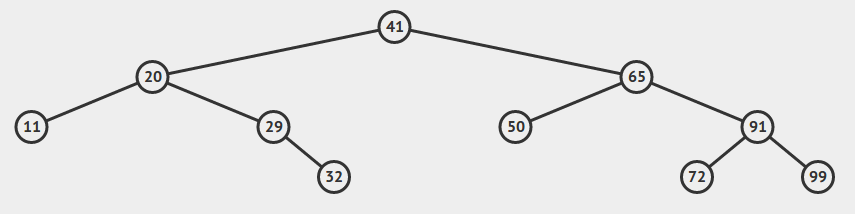
\includegraphics[width=0.8\textwidth]{img/BST}
  \end{center}
  \begin{itemize}
  \item \emph{Search Trees} Keep items in an ordered relationship.
  \item For example: Left children always have smaller values, Right
    children always have larger values;
  \item Insertion/Search/Deletion in a tree costs $O(h)$, where $h$ is
    the height of the tree;
  \item For a tree with $n$ elements, the \structure{minimum} height
    is $\text{log}n$
  \item For a balanced tree, the \structure{maximum} height is also
    $\text{log}n$
  \item How to keep the tree balanced?
  \end{itemize}
\end{frame}

\begin{frame}
  \frametitle{Balanced Search Trees}
  \framesubtitle{How to keep the tree balanced?}

  There are many Tree implementations/algorithms for keeping an BST
  balanced, and minimizing the tree height efficiently:
  \begin{itemize}
  \item AVL Tree (Adelson-Velskii-Landis);
  \item Red-Black Tree;
  \item B-Tree;
  \item Splay Tree;
  \end{itemize}
  \bigskip

  However, in a programming context (or even day to day life),
  implementing these trees from scratch is \alert{Dangerous}.

  \bigskip

  Luckly, most standard libraries include some implementation of BST.
\end{frame}

\begin{frame}
  \frametitle{ABLs in C++: Map and Set}

  \begin{itemize}
  \item In C++, the \emph{Map} and \emph{Set} classes are implemented
    using BSTs
  \item \emph{Map} Accept Key-value pairs;
  \item \emph{Set} Accepts only Keys;
  \end{itemize}

\end{frame}

\begin{frame}[fragile]
  \frametitle{Using Map in C++}
  {\small
\begin{verbatim}
#include <map>
map<string, int> ages;   ages.clear();

ages["john"] = 40;
ages["billy"] = 39;
ages["andy"] = 29;
ages["steven"] = 42;
ages["felix"] = 33;

// What is the age of andy?
map<string, int>::iterator it = ages.find("andy");
cout << it->second << endl;

// Which names are between "f" and "m" ??
for (map<string, int>::iterator it =
     age.lower_bound("f");              // finds felix
     it != age.upper_bound("m"); it++)  // finds johm
        cout << " " << ((string)it->first).c_str();
\end{verbatim}}
\end{frame}


\begin{frame}[fragile]
  \frametitle{Using Set in C++}
  {\small
\begin{verbatim}
#include <set>
set<int> CDs;
CDs.clear();

// Adding some values
CDs.insert(1000); CDs.insert(999); CDs.insert(1337);
CDs.insert(1313); CDs.insert(100020);

// Testing if a particular value exists (O(logn))
set<int>::iterator f = used_values.find(79);
if (f == used_values.end())
  cout << "not found!\n";
else
  cout << *f;    // Index!
\end{verbatim}}
\end{frame}

\subsection{Hash Tables}
\begin{frame}[fragile]
  \frametitle{Hash Tables}

  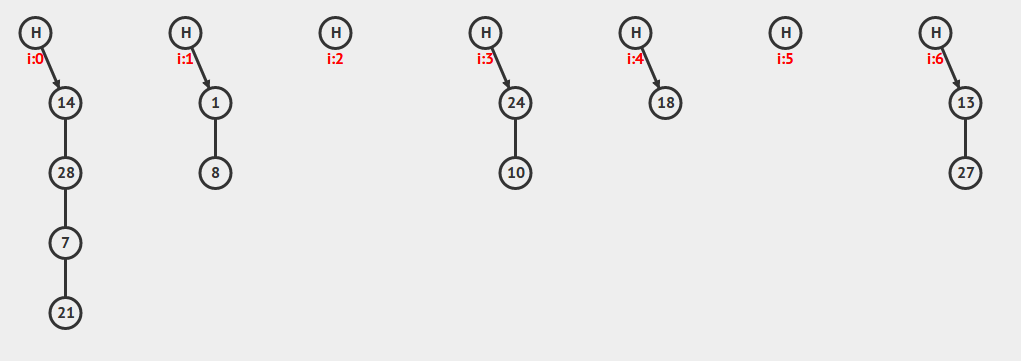
\includegraphics[width=0.95\textwidth]{img/hash}

  \begin{itemize}
  \item Insertion and Search: \structure{O(1)} -- \alert{Slow iteration};
  \item C++ library: \emph{std::unordered\_map};
  \item \structure{Hash} parameter -- Defines Collision results.
  \item Learn more about hash tables here: \url{https://visualgo.net/ja/hashtable}
  \end{itemize}
\end{frame}
